\documentclass{article}
\usepackage{tikz}
\usetikzlibrary{shapes.geometric,positioning}

\begin{document}

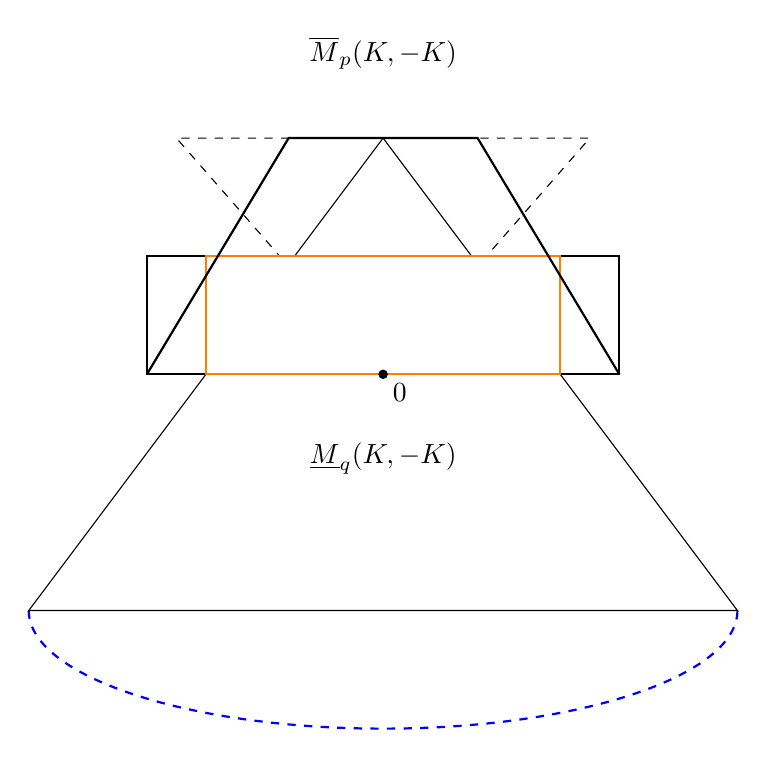
\begin{tikzpicture}[scale=1.5]
    % Draw the main triangle
    \draw[fill=white] 
        (-3,0) -- (0,4) -- (3,0) -- cycle;
    
    % Draw the inner dashed triangle
    \draw[dashed] 
        (0,2) -- (1.75,4) -- (-1.75,4) -- cycle;
    
    % Draw the black rectangle
    \draw[thick,black] 
        (-2,2) rectangle (2,3);
    
    % Draw the blue annulus
    \draw[thick,blue,dashed] 
        (-3,0) arc (180:360:3 and 1);
    
    % Draw the orange rectangle
    \draw[thick,orange,fill=white] 
        (-1.5,2) rectangle (1.5,3);
    
    % Draw the black lines forming the intersection
    \draw[thick,black] 
        (-2,2) -- (-0.8,4) -- (0.8,4) -- (2,2);

    % Label the origin
    \filldraw[black] (0,2) circle (1pt) node[below right] {$0$};
    
    % Add labels
    \node at (0,4.5) [above] {$\overline{M}_{p}(K,-K)$};
    \node at (0,1.5) [below] {$\underline{M}_{q}(K,-K)$};
    
\end{tikzpicture}

\end{document}